\section{\tool{} Design and Implementation}

The middle-end of a compiler is an exercise in compromises.
%
Much high-level language information, especially about types and about
structured control flow, has been thrown away.
%
At the same time, the target platform is frustratingly out of reach,
and it is difficult or impossible to take advantage of processor-level
tricks such as conditional execution and special-purpose instructions.


So, why have we developed a new middle-end superoptimizer?
%
First, LLVM IR is the narrow waist in a large and growing ecosystem of
frontends and backends; improvements made at this level can benefit
many projects and billions of end users (via, for example, Android).
%
Second, \tool{} excels at generating constants, particularly for
Boolean valued variables that are used to control branches.
%
Constants ripple through the rest of the middle-end and the full benefits are
not realized until constant propagation, dead code elimination, and other
optimization passes have exploited them.
%
Generating constants in the backend would leave these benefits on the
table.
%
Third, the SSA form that many modern compilers use in their middle
ends is effectively a functional programming language~\cite{Appel98}
that is highly amenable to automated reasoning techniques.


\subsection{An IR for Superoptimization}
\label{sec:ir}

\begin{figure}
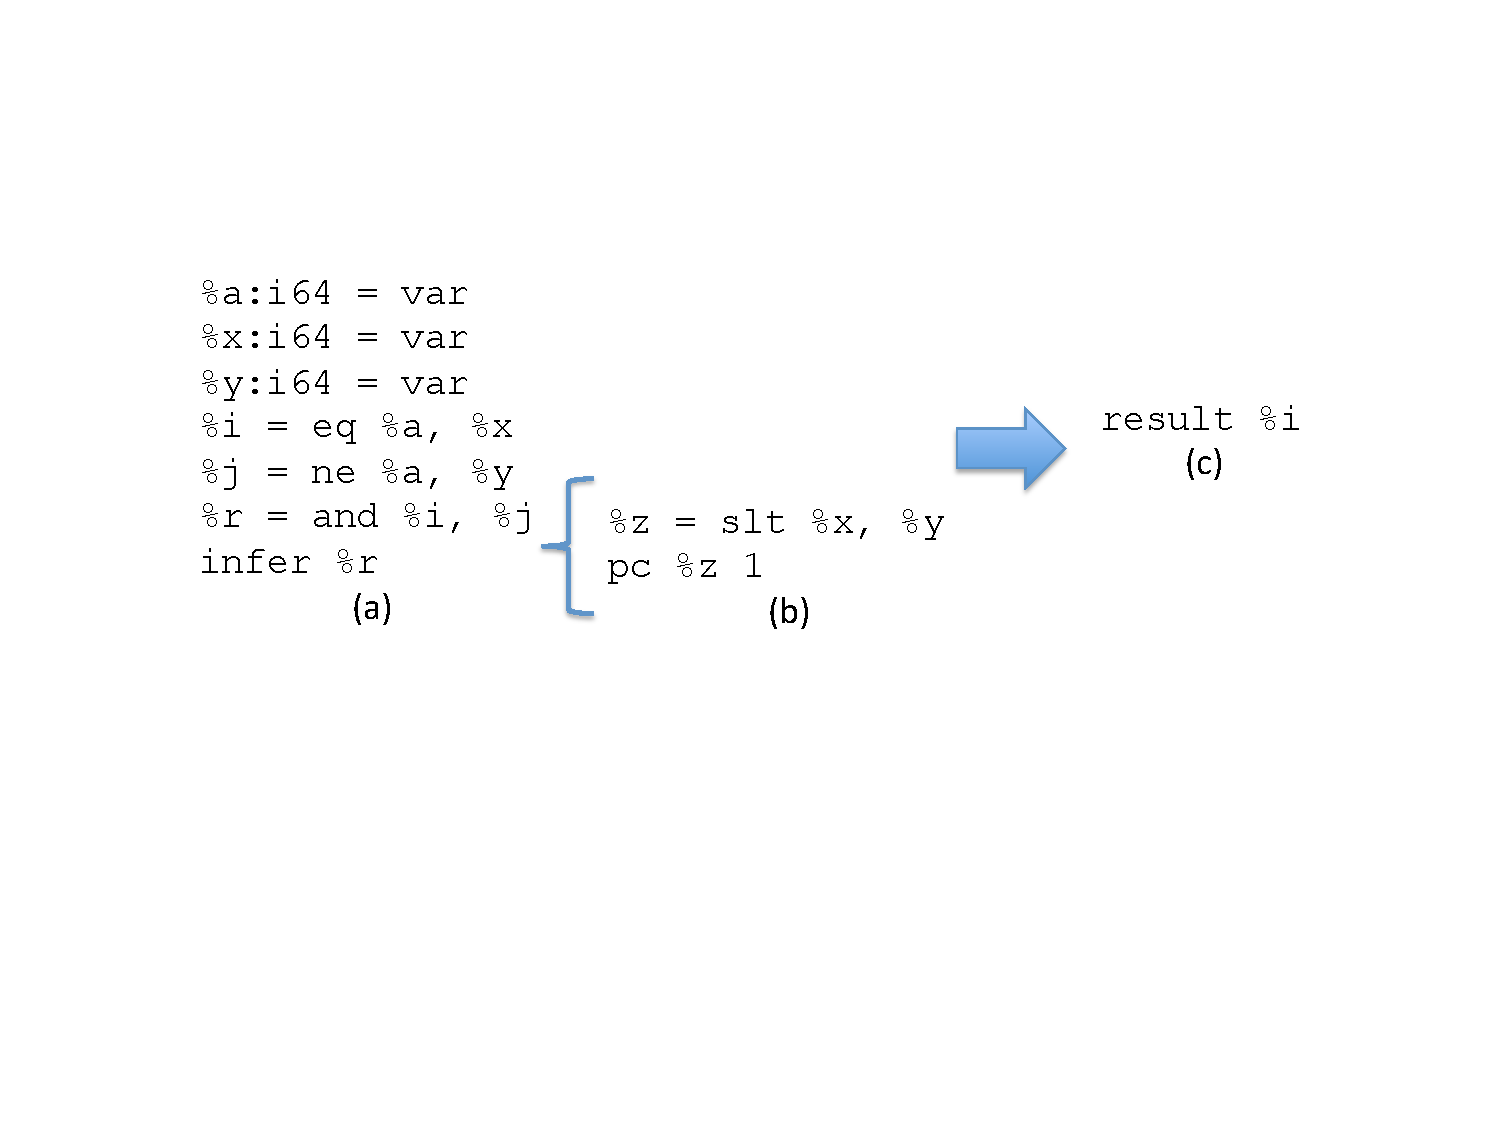
\includegraphics[width=\columnwidth]{figs/fig1.pdf}
  \caption{A simple \tool{} optimization. The left-hand side in (a)
    does not optimize.  Adding the path condition in (b) allows
    \tool{} to synthesize the right-hand side (c).}
  \label{fig:example1}
\end{figure}

\tool{}'s basic abstraction is a directed acyclic dataflow graph.
%
Operations closely follow those in the LLVM
IR,\footnote{\url{http://llvm.org/docs/LangRef.html}} though \tool{}'s
IR is purely functional.
%
\tool{} has 51 instructions, all derived from equivalents in the
integer, scalar subset of the LLVM instruction set.


The order of statements in \tool{} IR matters only in that a value
may not be referenced before it is defined.
%
An operand is either an integer constant or a value.
%
Integer constants have explicit widths; for example, the largest
signed 8-bit value is \texttt{127:i8}.
%
Constants may be either signed or unsigned, but this is only a
notational convenience: \tool{}, like LLVM and like processors,
associates signedness information with instructions rather than with
variables.
%
The only data types are bitvector, tuple of bitvector, and a special
block type.
%
Most operations are polymorphic with respect to bit width, and a few
type constraints are enforced:
%
\begin{itemize}
\item
  All bitvectors are at least one bit wide
\item
  Operand widths for instructions such as \texttt{add} must match
\item
  Comparison instructions return a single bit, and the first argument
  to a \texttt{select} instruction---LLVM's version of the ternary
  \texttt{?:} operator in C and C++---must be one bit wide
\item
  The \texttt{sext} (sign extend) and \texttt{zext} (zero extend)
  instructions must extend their argument by at least one bit
\item
  The \texttt{trunc} (truncate) instruction must reduce the bitwidth of its
  argument by at least one bit
\item
  Checked math operations such as \texttt{uadd.with.overflow} return
  a tuple consisting of the possibly-wrapped result and a bit
  indicating whether overflow occurred
\item
  The \texttt{extractvalue} instruction, like its LLVM counterpart,
  extracts a bitvector from a tuple
\end{itemize}
%
\tool{} does not perform type inference, but widths can be omitted in
most situations where they are obvious from context.


\subsection{Left-Hand Sides, Right-Hand Sides, and Path Conditions}

\tool{} does not have control flow, though it does provide two
constructs for representing dataflow facts learned from control flow
in the program being optimized.
%
%%% rsas: would it be better to add bit widths to all instructions
%%%       in Figure 1? %i:i1, %j:i1, etc.
%
For example, Figure~\ref{fig:example1}(a) shows the \emph{left-hand
  side} (LHS) of a potential optimization: the \texttt{infer} keyword
indicates the root node that \tool{} is being asked to optimize the
computation of.
%
Here \var{r} is a Boolean value that is true when the 64-bit input
\var{a} is equal to \var{x} and unequal to \var{y}.
%
In this case, \tool{} is unable to synthesize a better way to compute
\var{r}.


Now assume this left-hand side is augmented with the fact that \var{x}
is less than \var{y} using a signed comparison.
%
In \tool{}, such a fact is encoded as a path condition---an assertion
that a variable holds a particular value, that typically comes from
executing through a conditional branch in a program---that is shown in
Figure~\ref{fig:example1}(b).
%
Given this additional information, \tool{} can prove that \var{r} is
true if \var{a} equals \var{x}, and therefore the second comparison
and the \texttt{and}-instruction are unnecessary and can be dropped.
%
\tool{} represents a synthesis result as a \emph{right-hand side}
(RHS) containing the \texttt{result} keyword.
%
A right-hand side is a DAG that may refer to values on its
corresponding left-hand side.
%
A RHS is useful if it is cheaper to compute than its LHS\@.


A left-hand and right-hand side can be concatenated to create a
\emph{complete optimization}.
%
When presented with such an optimization, \tool's role is not to
synthesize, but rather to verify the correctness of the
optimization---a relatively straightforward job.


\subsection{Exploiting Correlated Phi Nodes}
\begin{figure*}
\begin{minipage}[b]{0.30\textwidth}
{\small\begin{verbatim}
int
f(bool cond, int z) {
  int x, y;
  if (cond) {
    x = 3 * z;
    y = z;
  } else {
    x = 2 * z;
    y = 2 * z;
  }
  return x + y;
}
\end{verbatim}}
\centering (a)
\end{minipage}
%
\begin{minipage}[b]{0.40\textwidth}
{\small\begin{verbatim}
define i32 @f(i1 %0, i32 %1) {
  br i1 %0, label %3, label %5

label %3:
  %4 = mul nsw i32 %1, 3
  br label %8

label %5:
  %6 = shl nsw i32 %1, 1
  %7 = shl nsw i32 %1, 1
  br label %8

label %8:
  %.07 = phi i32 [ %4, %3 ], [ %6, %5 ]
  %.0 = phi i32 [ %1, %3 ], [ %7, %5 ]
  %9 = add nsw i32 %.07, %.0
  ret i32 %9
}
\end{verbatim}}
\centering (b)
\end{minipage}
%
\begin{minipage}[b]{0.33\textwidth}
{\small\begin{verbatim}
%0 = block 2
%1:i32 = var
%2:i32 = shlnsw %1, 1:i32
%3:i32 = phi %0, %1, %2
%4:i32 = mulnsw 3:i32, %1
%5:i32 = phi %0, %4, %2
%6:i32 = addnsw %3, %5
infer %6
\end{verbatim}}
$\Rightarrow$
{\small\begin{verbatim}
%7:i32 = shl %1, 2:i32
result %7
\end{verbatim}}
\centering (c)
\end{minipage}
\caption{A C++ function that can be optimized to ``\texttt{return z <<
    2}'' (a), its representation in LLVM~IR (b), and a corresponding
  \tool{} LHS and RHS (c).  The first line of the LHS defines a block
  value with two predecessors; each phi node attached to this block
  will have two regular value arguments.  Then, the first argument to
  each phi node, \texttt{\%0}, establishes that they are correlated:
  since they come from the same basic block, they must make the same
  choice. Without information about the correlation between the phi
  nodes, this optimization cannot be synthesized.}
\label{fig:phi}
\end{figure*}


When control flow in LLVM code arrives at the start of a basic block,
each phi node~\cite{Cytron91} selects the value from its argument list
that corresponds to the block's immediate predecessor.
%
Lacking control flow, \tool{} preserves information about
correlated phi nodes using values of \emph{block type}.
%
Figure~\ref{fig:phi} shows an optimization that can only be performed
using the knowledge that two phi nodes make correlated choices.



\subsection{Reasoning About Incoming Control Flow}
\begin{figure*}
\begin{minipage}[b]{0.25\textwidth}
{\small\begin{verbatim}
unsigned
g(unsigned a) {
  switch (a % 4) {
  case 0:
    a += 3;
    break;
  case 1:
    a += 2;
    break;
  case 2:
    a += 1;
    break;
  }
  return a & 3;
}
\end{verbatim}}
\centering (a)
\end{minipage}
%
\begin{minipage}[b]{0.45\textwidth}
{\small\begin{verbatim}
define i32 @g(i32 %0) {
label %1:
  %2 = urem i32 %0, 4
  switch i32 %2, label %9 [
    i32 0, label %3
    i32 1, label %5
    i32 2, label %7
  ]

label %3:
  %4 = add i32 %0, 3
  br label %9

label %5:
  %6 = add i32 %0, 2
  br label %9

label %7:
  %8 = add i32 %0, 1
  br label %9

label %9:
  %.0 = phi i32 [ %0, %1 ], [ %8, %7 ],
                [ %6, %5 ], [ %4, %3 ]
  %10 = and i32 %.0, 3
  ret i32 %10
}
\end{verbatim}}
\centering (b)
\end{minipage}
%
\begin{minipage}[b]{0.33\textwidth}
{\small\begin{verbatim}
%0 = block 4
%1:i32 = var
%2:i32 = urem %1, 4:i32
%3:i1 = ne 0:i32, %2
%4:i1 = ne 1:i32, %2
%5:i1 = ne 2:i32, %2
blockpc %0 0 %3 1:i1
blockpc %0 0 %4 1:i1
blockpc %0 0 %5 1:i1
blockpc %0 1 %2 2:i32
blockpc %0 2 %2 1:i32
blockpc %0 3 %2 0:i32
%6:i32 = add 1:i32, %1
%7:i32 = add 2:i32, %1
%8:i32 = add 3:i32, %1
%9:i32 = phi %0, %1, %6, %7, %8
%10:i32 = and 3:i32, %9
infer %10
\end{verbatim}}
$\Rightarrow$
{\small\begin{verbatim}
result 3:i32
\end{verbatim}}
\centering (c)
\end{minipage}
\caption{A C or C++ function that can be optimized to ``\texttt{return 3}''
  (a), its representation in LLVM~IR (b), and the corresponding \tool{}
  LHS and RHS
  (c). The \tool{} IR has no control
  flow, but rather uses \texttt{blockpc} instructions to represent
  dataflow facts derived from converging control flow. These are
  crucial in giving \tool{} the information that it needs to
  synthesize the optimization.}
\label{fig:blockpc}
\end{figure*}


Consider the C function in Figure~\ref{fig:blockpc}(a).
%
In each case of the switch statement, \tool{} can use path condition
information extracted from control flow.
%
For example, the \tool{} LHS corresponding to the value of \texttt{a}
at the end of the first case (equivalently, corresponding to
\texttt{\%4} in Figure~\ref{fig:blockpc}(b)) is:

{\small\begin{verbatim}
%0:i32 = var
%1:i32 = urem %0, 4:i32
pc %1 0:i32
%2:i32 = add 3:i32, %0
infer %2
\end{verbatim}}

This asserts that at this program point, the remainder is zero.
%
The problem is that when we look at the program point where
information about the remainder values is actually useful---at the end
of \texttt{g}---we no longer have any path conditions, their
information has been lost as the control flow edges come together.
%
In other words, while path conditions capture useful information as
conditional branches are executed, they cannot represent facts about
convergent control flow.


To support reasoning about merged paths, \tool{} has a
\texttt{blockpc} construct: a reverse path condition tied to a value
of the block type.
%
The \tool~IR in Figure~\ref{fig:blockpc}(c) has six blockpcs, all tied
to block \texttt{\%0}.
%
The first, \texttt{blockpc \%0 0 \%3 1:i1}, asserts that when any phi
node tied to block \texttt{\%0} chooses its zeroth input, then
$\texttt{\%3} = 1$.
%
This fact, in turn, implies that \texttt{\%2}, the remainder, is not
equal to zero.
%
The next two blockpcs establish that the remainder is not one or two.
%
Together, these three conditions constrain the implicit default case
of the switch operator, which is the case where the remainder is three.
%
The next three blockpcs respectively constrain the three explicit
switch cases.
%
The overall effect is that \tool{} is able to reassemble information
learned in the switch cases in such a way that it is feasible to
derive the overall optimization.


\subsection{Extracting \tool{} IR from LLVM IR}

Since \tool{} has its own IR, it can run as a standalone tool.
%
However, we commonly want to convert LLVM IR into \tool{} IR on the fly, in
order to look for optimizations that can be applied to programs that we care
about.
%
For this purpose \tool{} uses LLVM's APIs to access the in-memory
representation of its IR\@.


\tool's \emph{extractor} scans each instruction in an LLVM module---a collection
of functions roughly equivalent to a C or C++ compilation unit---looking for
those that return integer-typed values.
%
Each such instruction leads to the construction of, and is the root
of, an \tool{} left-hand side.
%
The rest of the left-hand side is constructed by recursively following backwards
dataflow edges from this root instruction.
%
As the backwards traversal passes conditional branches and phi nodes
it adds path conditions and blockpcs.


To remain sound in the presence of loops, \tool{} must not extract any program
point more than one time in a single left-hand side.
%
In the vast majority of cases, LLVM's built-in loop detection suffices, but LLVM
does not detect irreducible loops, which occur rarely but which \tool{} must
detect on its own.
%
\tool{}'s backwards traversal is also stopped when it reaches a value
that comes from another function, a load from memory, or an
instruction that \tool{} lacks a model for, such as a floating point
or vector instruction.

Extraction is accompanied by canonicalization; arguments to
commutative operations are sorted; \tool{} canonicalizes away as many
comparison instructions as possible, for example turning greater-than
into less-than and swapping the operands; BitCast, PtrToInt, and
IntToPtr instructions simply pass on their bitvector values, throwing
away LLVM-level type information; GetElementPointer, LLVM's struct and
array element address generation instruction, is reduced to adds and
multiplies.


\subsection{Intrinsics}

We implemented 10 LLVM intrinsics as \tool{} instructions:
\begin{itemize}
\item
  Six operations that perform integer math while checking for
  overflow: there are signed and unsigned variants of add, subtract,
  and multiply
\item
  \texttt{ctpop}: Hamming weight
\item
  \texttt{bswap}: byte swap
\item
  \texttt{cttz} and \texttt{ctlz}: count trailing and leading zeroes
\end{itemize}

Combining several of these intrinsics, here \tool{} proves that the
Hamming weight of an arbitrary 64-bit value, multiplied by its number
of trailing zeroes, cannot overflow.

{\small\begin{verbatim}
%0:i64 = var
%1:i64 = ctpop %0
%2:i64 = cttz %0
%3 = smul.with.overflow %1, %2
%4 = extractvalue %3, 1
infer %4
\end{verbatim}}
$\Rightarrow$
{\small\begin{verbatim}
result 0:i1
\end{verbatim}}

The prevalence of these instructions varies across programs but, for
example,
UBSan\footnote{\url{http://clang.llvm.org/docs/UndefinedBehaviorSanitizer.html}}
inserts a large number of overflow checks into a program as it is
being compiled, and we would like to remove as many of these as
possible.


\subsection{Verifying Optimizations and Supporting Undefined Behavior}

\tool{} can be used to verify an optimization that was derived by hand
or synthesized previously---perhaps by an untrusted solver or
untrusted organization.
%
\tool{} is capable, for example, of proving equivalence of the first three
implementations of Hamming weight listed on the Wikipedia
page,\footnote{\url{https://en.wikipedia.org/wiki/Hamming_weight}} after they
are compiled to LLVM and then extracted into \tool{}.
%
To handle the fourth implementation, \tool{} would need to completely unroll the
loop, and to handle the fifth, it would need to model loads from a lookup table.



Verification follows the standard technique: \tool{} asks the solver
whether there exists any valuation of the inputs that causes
the left-hand and right-hand sides of the optimization to be unequal.
%
If this query is unsatisfiable, equivalence has been proved and
the optimization is sound.
%
If the query is satisfiable, a counterexample has been discovered and
it is presented to the user.
%
This is all fairly straightforward unless undefined behavior is
involved.


LLVM has three kinds of undefined behavior.
%
First, immediate undefined behavior, triggered by actions such as
dividing by zero or storing to an out-of-bounds memory location.
%
Second, an \emph{undef} value that stands for an indeterminate
register or memory location: it can return any value of its type.
%
Third, a \emph{poison} value that is more powerful than undef:
instructions other than \texttt{phi} and \texttt{select} return poison
if any input is poison.
%
Phi and select only return poison if the selected input is poison.
%
A poison value triggers true undefined behavior if it reaches a
side-effecting operation.


\tool{} does not model undef.
%
This is an acceptable approximation since undef usually occurs in the
context of uninitialized memory, and \tool{} has no model for memory.
%
When \tool{} encounters an explicit undef value while extracting
LLVM~IR into \tool{}~IR, it is conservatively modeled as zero.
%
Poison values are modeled by noting that any poison value in an \tool{}
expression will propagate to the root and trigger true undefined
behavior unless it is stopped by reaching the not-chosen input of a
phi or select instruction.
%
\tool{} models this behavior faithfully: each phi or select is
accompanied by an explicit path condition that only permits undefined
behavior to propagate via its selected branch.
%
The only immediate undefined behavior modeled by \tool{} is
divide-by-zero; \tool{} simply asserts to the solver that this does
not happen.


Some LLVM instructions have optional flags that add undefined behaviors.
%
For example, \texttt{add} is, by default, always defined, but
\texttt{add nsw} is undefined when signed overflow occurs, \texttt{add
  nuw} is undefined when unsigned overflow occurs, and \texttt{add nsw
  nuw} is undefined upon either kind of overflow.
%
\tool{} does not have flags, but rather provides separate instructions
corresponding to these different behaviors: \texttt{add},
\texttt{addnsw}, \texttt{addnuw}, and \texttt{addnswnuw}.
%
Similarly, the \texttt{exact} flag for division and right-shift, which
makes operations with remainders undefined, is modeled by supporting
\texttt{sdivexact} as well as \texttt{sdiv} and \texttt{ashrexact} as
well as \texttt{ashr}.


\subsection{Synthesizing Optimizations}

The essence of synthesis is finding a cost-minimizing solution to an
exists-forall formula.
%
In other words, we want to prove that there exists a way to connect up
a collection of instructions such that, for all inputs, the resulting
RHS behaves the same as its LHS\@.
%
Furthermore, the synthesized RHS should be the cheapest among all
that satisfy the behavioral requirement.


Given an equivalence checker, an algorithmically simple way to
implement synthesis is to enumerate, in order of increasing cost, all
RHSs, accepting the first one that passes the check.
%
In practice, this algorithm fails to produce results within an
acceptable amount of time when the cheapest RHS either contains
non-trivial constants or requires more than a handful of instructions.
%
To produce results in a more performant fashion, \tool{} uses
an improved version of the CEGIS (counterexample guided inductive
synthesis) algorithm developed by Gulwani et~al.~\cite{Gulwani11}.


CEGIS avoids exhaustive search and also avoids producing queries that
contain difficult quantifiers.
%
Rather, given a collection of instructions, it formulates a query
permitting all possible producer-consumer relations between
instructions, with the position of each instruction being represented
as a line number.
%
This query is satisfiable if there exists a way to connect the
instructions into a RHS that is equivalent to the LHS for just the
satisfying input.
%
If this is the case, the instructions and constants in the RHS can be
reconstructed from the model provided by the solver.
%
Then, in a second step, CEGIS asks the solver if the straight-line
program on the RHS is equivalent to the LHS for all possible inputs.
%
If so, synthesis has succeeded.
%
If not, constraints are added to prevent the solver from realizing
this particular circuit a second time, and the process is restarted.
%
In the worst case CEGIS is no better than naïve search, but in
practice it performs well, and has been shown to be capable of
generating RHSs of substantial complexity.
%
\tool{} wraps CEGIS in a second loop that constrains the size of the
synthesized RHS: it first attempts to synthesize a zero-cost RHS (no
new instructions are generated---the RHS may only use a constant or an
input), then a cost-one RHS (one instruction is generated), and so on.


Our improved CEGIS implementation can synthesize all \tool{} instructions
other than \texttt{phi}.
%
Using the \texttt{select} instruction, \tool{} can synthesize conditional
data paths.
%
Our algorithm is novel in that it can synthesize right-hand sides
composed of instructions that are polymorphic in the number of bits.
%
This requires \tool{} to augment the query with constraints that
enforce the bitwidth rules outlined in Section~\ref{sec:ir}.
%
A more difficult issue is that each instruction that is a candidate
for synthesis has a fixed bitwidth: there is no bitwidth-polymorphism
in the solver.
%
For each synthesis attempt, \tool{} starts with a default bitwidth:
the largest of any input and the target value.
%
Each instruction is instantiated at that width.
%
Next, for every input with a smaller bit width than the default bit
width, two extra components, a \texttt{zext} and a \texttt{sext}, are
instantiated that extend the input to the default width.
%
Finally, if the default width is larger than the output bit width of
the specification, \tool{} instantiates a \texttt{trunc} instruction
that truncates to the output width.
%
Similar transformations are applied to \texttt{select}'s conditional
input (\texttt{trunc}) and to the output of comparison instructions
 (\texttt{zext}).
%
These are heuristics and there is room for improvement.


\subsection{Validating \tool's Ability to Synthesize}

A synthesis implementation should be evaluated both in terms of
soundness and ability to synthesize a RHS when it exists.
%
We discuss soundness in more detail in Sections~\ref{sec:threats}
and~\ref{sec:validate}.
%
Regarding synthesis power, we ensured that \tool{} can synthesize a
subset of the ``Hacker's Delight'' optimizations from Gulwani et
al.~\cite{Gulwani11} where the instructions involved can be mapped to
\tool{}~IR in a one-to-one fashion and where the RHS is not too large
(P1--P17 and P19 out of P1--P25).
%
Our CEGIS implementation does not scale as well as Gulwani et al.'s,
we believe this is due to the extra synthesis components and constraints
relating to bitwidth rules.


We ensured that \tool{} can synthesize specific instances of every
optimization in Table~2 of Buchwald~\cite{Buchwald15}.
%
By ``specific instances,'' we mean that while Optgen can create a
general rule such as \texttt{\textasciitilde x + c} $\Rightarrow$ \texttt{(c - 1) - x}
that works for an arbitrary constant \texttt{c}, \tool{} must
rediscover the optimization for every bitwidth and every value of $c$
that appears in a program.


Finally, we validated \tool{}'s synthesis by ensuring that it can
solve discrete math problems.
%
Consider Mordell's equation, $y^2 = x^3 + k$, in the domain of natural numbers,
where $k$ is a constant.
%
We can encode a bounded version of this equation for $k = 7$, a case known
to not have any solutions, like this:
%
{\small\begin{verbatim}
%x:i32       = var
%y:i32       = var
%xsqr        = mulnuw %x, %x
%xcubed      = mulnuw %x, %xsqr
%ysqr        = mulnuw %y, %y
%xcubedplus7 = addnuw %xcubed, 7
%cmp         = eq %xcubedplus7, %ysqr
pc %cmp 1
infer %y
\end{verbatim}}

The ``nuw'' variants of multiplication and addition assert that unsigned integer
overflow is undefined, protecting us from undesirable wraparound effects.
%
The path condition asserts that the equation holds and the \texttt{infer} line
asks \tool{} for the value of $y$.
%
It fails to synthesize a RHS\@.


Similarly, \tool{} fails to synthesize a result when $k = 1$, because that case
has multiple solutions: $x=0$, $y=1$ and $x=2$, $y=3$.
%
On the other hand, for $k = 785$ there is a unique solution within the
bounds and \tool{} finds it:

{\small\begin{verbatim}
result 32146:i32
\end{verbatim}}
\noindent

\noindent
when asked to infer \texttt{\%x}:

{\small\begin{verbatim}
result 1011:i32
\end{verbatim}}

While we do not know of any use cases for solving Diophantine
equations inside an optimizing compiler, we are gratified to know that
the power is there should it be needed.


\subsection{Three Real Threats to Soundness}
\label{sec:threats}

We have observed miscompilations due to three causes other than the
obvious one (defects in \tool's implementation).
%
First, an incorrect LLVM optimization can turn a defined program into
an undefined one, but in a subtle way that is not exploited by an LLVM
backend.
%
There are known, long-standing bugs of this type in LLVM, and it is
difficult to get them fixed because their effects are difficult to
observe via end-to-end testing of the LLVM toolchain, and also because
the LLVM community has not reached consensus on exactly what the fix
should look like.
%
\tool{}, on the other hand, readily notices and exploits undefined
behaviors in order to perform computations more cheaply.
%
This is a highly unsatisfactory state of affairs, but fixing them
requires community-wide effort.
%
In the meantime, the problem can be mitigated by turning off some
problematic LLVM passes (SimplifyCFG, GVN, and InstCombine) or by
adjusting \tool{}'s LLVM semantics (using a command line option) to
prevent it from exploiting undefined behavior.


A second, closely related problem is that some applications
execute undefined behavior that happens to be benignly compiled by
LLVM\@.
%
In this case, the application, not LLVM, is wrong, but the end result
can be the same: \tool{} notices and exploits the undefined behavior
to break the application.
%
From this perspective, \tool{} might be viewed as a hostile
re-implementation of STACK~\cite{Wang13} that breaks programs instead
of providing helpful diagnostics.
%
This risk can be mitigated in two ways.
%
First, as above, UB exploitation in \tool{} can be disabled.
%
This is not a complete fix, but it does prevent some
particularly egregious problems.
%
Second, every UB exploited by \tool{} can be detected by LLVM's
undefined behavior
sanitizer.\footnote{\url{http://clang.llvm.org/docs/UndefinedBehaviorSanitizer.html}}
%
Developers should be using UBSan anyhow, since \tool{} is hardly the
worst problem faced by an undefined C or C++ program.


Third, when a solver is wrong, \tool{} will also be wrong.
%
One time we saw a program that had been optimized by \tool{}
misbehave, and the root cause was an incorrect result returned by the
Z3 solver.
%
We reported the bug and the Z3 developers rapidly fixed it.
%% \footnote{http://z3.codeplex.com/workitem/143}
%
Although we do not routinely check solvers against each other, we can
do so on demand since \tool's queries are in the SMT-LIB format
supported by most solvers.


\subsection{Validating Soundness}
\label{sec:validate}

Validating any particular optimization produced by \tool's synthesizer
is not difficult: each result that it creates can be verified by
\tool{}'s equivalence checker.
%
The equivalence checker is much simpler and we have more confidence in
it.


We validated \tool{}'s soundness in several ways.
%
First, we have stress-tested it using Csmith~\cite{Yang11} and also by
compiling significant programs, such as LLVM and SPEC CINT 2006,
that have good test suites.
%
Several SPEC benchmarks misbehave after being optimized by \tool{}
unless undefined behavior exploitation is disabled.
%
This is hardly surprising since some of these benchmarks are known to
execute undefined behaviors~\cite{Dietz15} and can even be broken by
GCC if the wrong optimization options are used.\footnote{The release
  notes for GCC~4.8 include this note: ``GCC now uses a more
  aggressive analysis to derive an upper bound for the number of
  iterations of loops using constraints imposed by language
  standards. This may cause non-conforming programs to no longer work
  as expected, such as SPEC CPU 2006 464.h264ref and 416.gamess. A new
  option, -fno-aggressive-loop-optimizations, was added to disable
  this aggressive analysis.''}
%
Some LLVM~3.9 test cases give the wrong answers when LLVM has been
optimized by \tool{}, even when undefined behavior exploitation is
turned off.
%
We believe these are due to undefined behaviors in LLVM, such as uses
of uninitialized storage, that cannot be easily mitigated just by
disabling undefined behavior exploitation in \tool{}.
%
We discuss this issue further in Section~\ref{sec:online}.
%
Second, we have validated \tool{} by looking at hundreds of
optimizations by hand, by posting optimizations on the web where LLVM
developers could see them, and by cross-checking them using
Alive~\cite{Lopes15}, which has an independent formalization of the
semantics of the LLVM instruction set.
%
In summary, we have made a good-faith attempt to validate \tool, but
it remains a research-quality optimizer that may well harbor exciting
bugs.


\subsection{Caching}
\label{sec:cache}

Since \tool{} must invoke a solver multiple times to synthesize an
optimization such as the ones shown in Figures~1--3, and since such
invocations often result in the solver being killed when a timeout
expires, we would like to amortize the costs of optimization
synthesis.
%
A reasonable solution is to cache the mapping of left-hand sides to
right-hand sides, including the null right-hand side indicating
failure to optimize.


\tool's first-level cache is a hash table in RAM, allowing very fast
lookups for commonly-occurring left-hand sides that are likely to be
encountered multiple times during a single compiler invocation.
%
\tool's second-level cache is Redis,\footnote{\url{http://redis.io/}} a fast,
networked key-value store.
%
\iffalse
As Figure~\ref{fig:example1}(a) suggests, serialized \tool{} IR is
somewhat verbose; a binary or compressed encoding would reduce cache
footprint and network traffic.
%
We have not yet implemented any such scheme since even for large
compilations, cache sizes have remained reasonable, in the range of a
few hundred MB at most.
\fi


\iffalse
\subsection{Limitations}
\label{sec:limit}

\tool{} does not reason about loops, pointers, the contents of memory,
floating point, or vector types.
%
We have instead chosen to focus on integer optimizations for variables
that LLVM is able to promote into SSA form.
\fi


\subsection{Implementation}
\label{sec:impl}

\tool{} is open source software and is implemented in about 9,500
lines of C++.
%
\tool{} currently links against LLVM~3.9.
%
\tool{}'s functionality can be invoked in a number of ways; there are
command-line tools for processing \tool{} IR and LLVM IR, and \tool{}
can be linked into a shared library that is dynamically loaded as an
LLVM optimization pass.
%
\tool{}'s LLVM pass registers itself using \texttt{EP\_Peephole}, an
extension point designed for peephole-like passes.
%
At the \texttt{-O2} or \texttt{-O3} levels, LLVM runs \tool{} five
times during compilation, giving it multiple opportunities to interact
with other optimization passes.
%
Finally, we have implemented a compiler driver \texttt{sclang} that is
a drop-in replacement for \texttt{clang} except that it loads the
\tool{} pass.
%
This makes it easy to build arbitrary software packages using \tool.



\tool{} uses Klee~\cite{Cadar08} as a library for emitting a query in SMT-LIB
format~\cite{Barrett10}.
%
By default, in order to model memory, Klee uses the theory of
bitvectors and arrays.
%
However, we observed that solvers such as Z3 can perform poorly in
this theory and also that \tool{} does not require a model for memory,
so we patched Klee to emit queries in the theory of quantified
bitvectors.


During the course of our work we ran into several degeneracies in Klee
triggered by, for example, large \tool{} LHSs with many phi nodes.
%
We fixed (and upstreamed) several issues, but in the end huge \tool{}
queries still performed poorly, triggering apparently exponential
behaviors.
%
We currently work around these issues by enforcing a limit on LHS
size: \tool{} simply drops any LHS that is over the specified limit,
which is configurable but defaults to 1\,KB of serialized IR\@.
%
This mechanism saves a lot of execution time while dropping a small
minority of queries.


\iffalse
\tool{} always spawns the solver in an external process, as opposed to
using the solver as a library.
%
There is, of course, overhead involved in creating a process,
serializing the query in \tool{}, and unserializing it in the solver.
%
Our judgment was the advantages of isolating the solver in a process
so that it could not crash \tool{}, and so that we could use the
operating system to limit its resource usage, out-weighted any
throughput improvements we might see from using the solver via an
in-process API\@.
%
Rather than making solver invocations fast, we rely on the caching
layers to amortize the costs.
\fi
